%! Author = joels
%! Date = 03/01/2021

\section{Responsive Design}
% Studierende können …
% - die folgenden Begriffe erklären:
    %Flexible Layout, Responsive Layout, Graceful Degration, Progressive Enhancement, Mobile First Layout, CSS Resets / CSS Normalization.
% - CSS Media-Queries erstellen.
% - Flexible Layout mit dem Box-Model erstellen, interpretieren und korrigieren. inklusive calc(), min(), max(), clamp(); position absolute/relative
% - Flexbox Layouts erstellen, interpretieren und korrigieren.
% - CSS Grid Layouts erstellen, interpretieren und korrigieren.
\textbf{\textcolor{blue}{Flexibles vs Responsives Layout:}}\\
\textbf{Flexible:} Dynamisches (grössenadaptives) Layout welches sich ohne Media-Queries umsetzen lassen. \textbf{Responsive:} Dynamisches Layout welches für unterschiedliche Geräte, Bereiche von Display-Grössen und unterschiedliche Medien separates ein Layouts definiert. $\rightarrow$ Umsetzung mit Media Queries\\
\textbf{Graceful Degradation:}  Baseline of full functionality available in modern browsers and then taking the layers off to ensure it works with older browsers.\\
\textbf{Progressive Enhancement:} Baseline of the features supported by all browsers and advanced features added like layers.\\
\textbf{Mobile first:} Base Layout und Design sind für Mobile
\subsection{Responsive Web layout}
\textbf{\textcolor{blue}{Media Queries:}}\\
\textbf{Typische Trigger Punkte:} (besser em verwenden)
\begin{itemize}[topsep=0pt, leftmargin=3mm]
    \setlength\itemsep{-0.3em}
    \item 480px/30em: Smartphones
    \item 768px/48em: Tablets
    \item 992px/62em: Desktops
\end{itemize}
\begin{lstlisting}[style=htmlcssjs]
// Typen
@media screen { ... }
@media print { ... }
// Dimensionen
@media ([width | min-width | max-width] : 375px { ... }
@media ([height | min-height | max-height] : 667px {...}
//Zustände
@media (orientation: landscape) { ... }
// Features
@supports not (display: grid) { div { float: right; } }
// Sonstiges
@media (hover: hover) { ... }
@media (pointer: fine | coase | none) { ... }
@media (any-pointer: fine | coase | none) { ... }
@media (min-resolution: 300dpi) { ... }
@media (min-color: 1) { ... }
// Operatoren
@media (min-width: 20em) and (max-width: 30em) { ... }
@media (max-width: 10em), (min-width: 20em) and (max-width: 30em), (min-width: 40em) { ... }
@media not screen { ... }
@media not screen and (min-width: 20em) { ... }
@media only screen { ... }
\end{lstlisting}
Link referenz mit media Attribut wird nur geladen wenn Bedingnung erfüllt:
\begin{lstlisting}[style=htmlcssjs]
<head> ...
  <link rel="stylesheet" href="LargeScreenLayout.css" media="(min-width: 30em)">
</head>
\end{lstlisting}
\textbf{\textcolor{blue}{View Port:}}\\
Mobile Geräte benötigen Viewport Meta-Tag Spezifikation,für die Skalierung:
\begin{lstlisting}[style=htmlcssjs]
<meta name="viewport" content="width=device-width,initial-scale=1">
\end{lstlisting}
\subsection{Flexible Layout}
\textbf{\textcolor{blue}{Box-Model}}\\
\begin{minipage}{0.63\linewidth}
    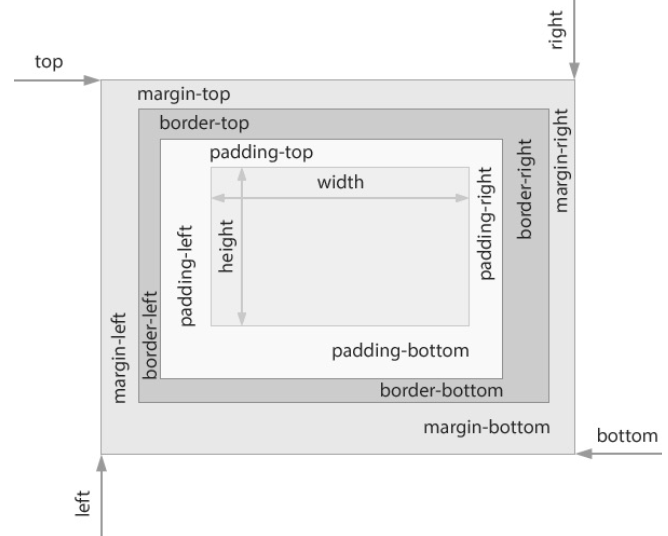
\includegraphics{media/css_display.png}
\end{minipage}
\begin{minipage}{0.37\linewidth}
    Box-Sizing Model gilt nur, wenn display \textcolor{blue}{block} oder \textcolor{blue}{inline-block}\\
    Zentrieren von Elementen: max-width: 50em; margin 0 auto;
\end{minipage}
\textbf{\textcolor{blue}{CSS FUnktionen:}}
\begin{lstlisting}[style=htmlcssjs]
width: calc(100vw - 5em); // 100vw = 100% der View Width
width: min(500px, 100vW - 5em);
width: max(400px, 100vw - 5em);
width: clamp(400px, 100vw - 5em, 500px); // Links: untere Grenze, Mitte: Bevorzugt, Rechts: obere Grenze
\end{lstlisting}
\textbf{\textcolor{blue}{Was bedeutet 100\%?}}\\
\textbf{Parent's height:} height, top\\
\textbf{Parent's width:} width, left, margin-top, margin-left, padding-top, padding-left\\
\textbf{Self's height:} translate-top\\
\textbf{Self's width:} translate-left\\
\textbf{\textcolor{blue}{Scrolling/Overflow:}} overflow: visible | hidden | scroll\\
\textbf{visible:} Text über Box hinaus\\
\textbf{hidden:} Text abgeschnitten/nur in Box\\
\textbf{scroll:} Scrollbar (oft erst bei Interaktion)\\
\textbf{\textcolor{blue}{Werte von Position:}}
\begin{itemize}[topsep=0pt, leftmargin=3mm]
    \setlength\itemsep{-0.3em}
    \item absolute: Element aus dem Element-Fluss entfernt\\
    - Eigenschaften: top, left, bottom, right, width, height (Werte relativ zum ersten Parent mit position: relative/absolute)\\
    - Erlaubt Überlappung von Elementen
    \item fixed: Immer am gleichem Ort
    \item sticky: Box bleibt am oberen (oder unteren) Rand des Fensters haften
    \item static: Standard-Positionierung im Fluss
    \item relative: Platz im Fluss bleibt reserviert
\end{itemize}
\subsubsection{Flexbox}
\begin{itemize}[topsep=0pt, leftmargin=3mm]
    \setlength\itemsep{-0.3em}
    \item display: flex;
    \item Betrifft alle direkten Kind-Elemente = \dq Flex-Items\dq
    \item Inline Styling ist nicht empfohlen
    \item Alle Flex-Items verhalten sich wie \dq inline blocks\dq $\rightarrow$ Können \textcolor{blue}{height} und \textcolor{blue}{width} definieren
\end{itemize}
\textbf{\textcolor{blue}{Grösse:}}\\
Flex-Items definieren individuell wie sie mit verfügbarem Platz in der \dq Main-Axis\dq umgehen\\
\textbf{flex-grow:} Verhältnis wie der Platz verteilt wird $\rightarrow$ Default: 0 (nicht grösser werden)\\
\textbf{flex-shrink:} Verhältnis, wie die Elemente kleiner werden wenn zu wenig platz $\rightarrow$ Default: 0\\
\textbf{Kurzform:} flex: [flex-grow][flex-shrink][flex-basis] (default: 0, 0, auto)\\
$\rightarrow$ Wenn alle Flex-Items \textbf{flex-grow: 0} und \textbf{margin: auto} haben, ist eine Verteilung des leeren Platzes notwendig. Wird auf dem Container definiert: \textbf{justify-content: flex-start | flex-end | center | space-between | space-around}\\
\textbf{\textcolor{blue}{Wrap:}}\\
$\rightarrow$ Definiert auf Container und wrappt eine Elemente sinnvoll.\\
\textbf{flex-wrap: wrap} ignoriert flex-shrink Definitionen der Flex-Items. Pro Zeile Verteilung entsprechend flex-grow oder justify-content\\
\textbf{\textcolor{blue}{Order:}} order: 1
\begin{itemize}[topsep=0pt, leftmargin=3mm]
    \setlength\itemsep{-0.3em}
    \item Flex Elemente werden entsprechend \dq source order\dq platziert
    \item Verwendet, um reihenfolge der Elementa anzupassen
    \item Kann auch negativ sein (Default: 0)
    \item Nicht \dq accessible\dq: reihenfolge für Screen reader ändert nicht
\end{itemize}
\textbf{\textcolor{blue}{Flex-Direction:}}\\
\textbf{flex-direction: row | row-reverse | column | column-reverse}
\begin{itemize}[topsep=0pt, leftmargin=3mm]
    \setlength\itemsep{-0.3em}
    \item Default: row
    \item Ändert die Haupt-Layoutrichtung
    \item Bei \textcolor{blue}{flex-direction: column} braucht Container eine Höhe
    \item Bei \textcolor{blue}{row-reverse} und \textcolor{blue}{column-reverse} kennen CSS Selektoren nur die source order
\end{itemize}
\textbf{\textcolor{blue}{Höhe, Breite, Ausrichtung:}}\\
Default: FlexBox-Items füllen den Platz horizontal (Main Axis) und vertikal (Cross Axis) aus (flex-direction: row)\\
\textbf{Main-Axis:} Für Items: Attribut \textcolor{blue}{flex}, für Container: Attribut \textcolor{blue}{justify-content}\\
\textbf{Cross-Axis:} Für Container: \textcolor{blue}{align items: stretch | flex-start | flex-end | center | baseline}, für Items: \textcolor{blue}{align-self}\\
\textbf{\textcolor{blue}{Summary:}}\\
\textbf{Container Eigenschaften:}
\begin{itemize}[topsep=0pt, leftmargin=3mm]
    \setlength\itemsep{-0.3em}
    \item Hauptachse (main axis) wählen:\\
    flex-direction: row | column
    \item Mehrzeilig erlaubt? (wrap):\\
    flex-wrap: nowrap | wrap
    \item Alignment entlang der Hauptachse wählen (wenn nötig):\\
    justify-content: flex-start | flex-end | center | space-around | space-between
    \item Alignment entlang der Querachse (cross axis) wählen (wenn nötig):\\
    align-items: stretch | flex-start | flex-end | center
\end{itemize}
\textbf{Item Eigenschaften:}
\begin{itemize}[topsep=0pt, leftmargin=3mm]
    \setlength\itemsep{-0.3em}
    \item Dynamische Grössenveränderung (Hauptachse):\\
    flex: [flex-grow] [flex-shrink] [flex-basis] (z.B. 0 0 0)
    \item Alignment des Elements entlang der Querachse (cross axis):\\
    align-self: flex-start | flex-end | center | stretch | auto
\end{itemize}
\subsubsection{CSS Grid}
\textbf{Auf Grid Container:} \textcolor{blue}{display: grid}\\
\textbf{\textcolor{blue}{Grösse:}}\\
\textbf{fr:} Freier Platz wird aufgeteilt. fr Spalten können nicht schmaler als das längste Wort werden.\\
\textbf{min-content:} Soviel Platz in der Breite wie das längste Wort benötigt.
\textbf{max-content:} Soviel Platz in der Breite wie der gesamte Text auf einer Zeile benötigt.
\textbf{\textcolor{blue}{Template:}}\\
\textbf{Definition:} grid-template-columns, grid-template-rows, grid-template-areas\\
\textbf{Platzierung:} grid-[column|row]-[start|end]: number\\
\textcolor{blue}{Kurzform:} grid-column: 1/5, grid-row: 1/2 (start/end)\\
\textcolor{blue}{Alle 4:} grid-area: Y1/X1/Y2/X2;
\begin{lstlisting}[style=htmlcssjs]
// Beispiele:
grid-template-columns: auto 7em 1fr minmax(2em, 20em);
grid-row-start: 1; grid-row-end: 2;
grid-area: 1/1/2/5
\end{lstlisting}
\textbf{\textcolor{blue}{Alignment:}}\\
\textbf{Y-Achse}\\
\textbf{Default:} align-items: stretch; (Items nehmen die ganze Höhe der Zeile an.)\\
\textbf{Alternativen:}
\begin{itemize}[topsep=0pt, leftmargin=3mm]
    \setlength\itemsep{-0.3em}
    \item Oben: align-items: start;
    \item Mitte: align-items: center;
    \item Unten: align-items: end;
    \item Anpassung per Item statt auf Container: align-self
\end{itemize}
\textbf{X-Achse:}\\
\textbf{default:} justify-items: stretch; (Items nehmen die ganze Breite der Zelle ein.)\\
\textbf{Alternativen:}
\begin{itemize}[topsep=0pt, leftmargin=3mm]
    \setlength\itemsep{-0.3em}
    \item Links: justify-items: start;
    \item Mitte: justify-items: center;
    \item Rechts: justify-items: end;
    \item Anpassung per Item statt auf Container: justify-self
\end{itemize}















